\documentclass[12pt,a4paper]{article}
\usepackage[utf8]{inputenc}
\usepackage[russian]{babel}
\usepackage{amsmath, amssymb, amsfonts}
\usepackage{graphicx}
\usepackage{float}
\usepackage{geometry}
\geometry{left=2.5cm, right=2cm, top=2cm, bottom=2cm}
\usepackage{indentfirst}
\usepackage{caption}
\usepackage{xcolor}
\usepackage{multirow}

\begin{document}


\title{\begin{center}Лабораторная работа № 5.5.1\end{center}
Измерение коэффициента ослабления потока $\gamma$-лучей в веществе и определение их энергии}
\author{Струков О. И. \\ Б04-404}
\date{}

\thispagestyle{empty}
\pagenumbering{gobble}
\maketitle
\newpage
\pagenumbering{arabic}

\section*{Теоретическая часть}

Гамма-кванты представляют собой электромагнитное излучение, возникающее при переходе возбуждённых атомных ядер из одного энергетического состояния в другое, более низкое. Энергия $\gamma$-квантов обычно лежит в диапазоне от нескольких десятков кэВ до нескольких МэВ. Поскольку гамма-кванты не обладают электрическим зарядом, а их масса покоя равна нулю, они не испытывают кулоновского торможения и взаимодействуют с веществом лишь посредством трёх основных процессов: \textbf{фотоэффекта}, \textbf{комптоновского рассеяния} и \textbf{рождения электрон-позитронных пар}.

\subsection*{Основные процессы взаимодействия $\gamma$-излучения с веществом}

\textbf{Фотоэлектрическое поглощение (фотоэффект).} При столкновении $\gamma$-кванта с электроном внутренней атомной оболочки может происходить полное поглощение кванта. Энергия фотона передаётся электрону, а импульс распределяется между этим электроном и ионом. Свободный электрон поглотить $\gamma$-квант не может, так как при этом невозможно одновременно удовлетворить законам сохранения энергии и импульса. Наружные электроны также не принимают участия в фотоэффекте, поскольку они слабо связаны в атоме и их практически можно считать свободными.

Вероятность $dP$ фотоэлектрического поглощения пропорциональна длине пути $dl$ и плотности внутренних электронов в среде:
\begin{equation}
    dP = \sigma \, n_1 \, dl,
    \label{eq:photo_prob}
\end{equation}
где $n_1$ --- плотность внутренних электронов, а $\sigma$ --- поперечное сечение фотоэлектрического поглощения, рассчитанное на один электрон. Связь между коэффициентом поглощения $\mu_\text{ф}$ и сечением $\sigma$ имеет вид:
\begin{equation}
    \mu_\text{ф} = \sigma \, n_1.
    \label{eq:photo_mu}
\end{equation}
Вероятность фотоэффекта сложным образом зависит от энергии $\gamma$-лучей и заряда ядра $Z$. Для оценок можно пользоваться соотношением:
\begin{equation}
    \sigma \propto \frac{Z^5}{(\hbar\omega)^{3{,}5}}.
    \label{eq:photo_sigma}
\end{equation}
Из этой формулы видно, что вероятность фотоэффекта быстро возрастает при переходе от лёгких к тяжёлым элементам и резко падает с увеличением энергии $\gamma$-квантов. Фотоэффект является доминирующим механизмом поглощения при не очень высоких энергияях.

\textbf{Комптоновское рассеяние.} Комптоновским рассеянием (или комптон-эффектом) называется упругое столкновение $\gamma$-кванта с электроном. При таком столкновении $\gamma$-квант передаёт электрону часть своей энергии, величина которой определяется углом рассеяния. В отличие от фотоэффекта, который может идти только на сильно связанных электронах, комптоновское рассеяние происходит на свободных или слабосвязанных электронах. Атомные электроны в этом случае можно считать практически свободными.

Сечение комптон-эффекта $\sigma_K$, отнесённое к одному свободному электрону, при энергиях $\gamma$-кванта, много больших энергии покоя электрона, принимает вид:
\begin{equation}
    \sigma_K = \pi r_e^2 \frac{m c^2}{\hbar\omega} \left( \ln \frac{2\hbar\omega}{m c^2} + \frac{1}{2} \right),
    \label{eq:compton_sigma}
\end{equation}
где $r_e \approx 2{,}8 \cdot 10^{-13}$ см --- классический радиус электрона, а $m$ --- его масса. Сечение $\sigma_K$ с ростом энергии фотонов падает далеко не так резко, как сечение фотоэффекта. Комптоновский коэффициент линейного ослабления $\mu_K$ связан с сечением $\sigma_K$ формулой, аналогичной~\eqref{eq:photo_mu}, где под $n$ следует понимать полную плотность электронов в веществе. Важно отметить, что, в отличие от фотоэффекта, эффект Комптона приводит не к поглощению $\gamma$-квантов, а к их рассеянию и уменьшению их энергии.

\textbf{Образование электрон-позитронных пар.} При энергиях $\gamma$-лучей, превышающих $2mc^2 = 1{,}022$ МэВ, становится возможным процесс поглощения $\gamma$-лучей, связанный с образованием электрон-позитронных пар. Рождение пары не может происходить в вакууме, оно возникает в электрическом поле ядер. Вероятность этого процесса приблизительно пропорциональна $Z^2$ и сложным образом зависит от энергии фотона. При энергиях, с которыми приходится иметь дело в ядерной физике, рождение пар существенно только в самых тяжёлых элементах. Так, даже для свинца вероятность рождения пар сравнивается с вероятностью комптоновского эффекта только при энергии около $4{,}7$ МэВ.

\subsection*{Закон ослабления узкого пучка $\gamma$-лучей}

Полный линейный коэффициент $\mu$ ослабления пучка $\gamma$-квантов при прохождении через вещество равен сумме коэффициентов для всех трёх рассмотренных процессов:
\begin{equation}
    \mu = \mu_\text{ф} + \mu_K + \mu_\text{п}.
    \label{eq:mu_total}
\end{equation}

Рассмотрим опыты, поставленные в хорошей геометрии, то есть в условиях, когда исследуется прохождение через вещество узкого параллельного пучка $\gamma$-лучей. В этом случае не только фотоэлектрическое поглощение и генерация пар, но и комптоновское рассеяние выводят $\gamma$-кванты из пучка. Поэтому при прохождении через вещество меняется только количество, но не энергия $\gamma$-квантов в пучке, так что коэффициент $\mu$, характеризующий поглощение $\gamma$-квантов в веществе, не зависит от длины пути. Обозначим через $-dN$ число $\gamma$-квантов, выбывших из пучка на пути $dl$. Это число пропорционально имеющемуся их числу $N$ и пройденному пути $dl$:
\begin{equation}
    -dN = \mu N \, dl.
    \label{eq:diff_eq}
\end{equation}
Интегрируя уравнение~\eqref{eq:diff_eq} от нулевой толщины до заданной, получим экспоненциальный закон ослабления:
\begin{equation}
    N = N_0 \, e^{-\mu l},
    \label{eq:attenuation}
\end{equation}
где $N_0$ --- число $\gamma$-квантов, падающих на поглотитель, а $N$ --- число квантов, прошедших через слой вещества толщиной $l$.

Закон~\eqref{eq:attenuation} может быть записан в двух эквивалентных формах:
\begin{equation}
    I = I_0 \, e^{-\mu l}, \qquad I = I_0 \, e^{-\mu' m_1},
    \label{eq:two_forms}
\end{equation}
где $I$, $I_0$ --- интенсивности прошедшего и падающего излучений, $l$ --- длина пути, пройденная пучком $\gamma$-лучей, $m_1$ --- масса пройденного вещества, приходящаяся на единицу площади. Величина $\mu$ имеет размерность см$^{-1}$, а $\mu'$ --- см$^2$/г. Форма записи с $\mu'$ является предпочтительной, поскольку $\mu'$, в отличие от $\mu$, не зависит от плотности среды.

Из формулы~\eqref{eq:attenuation} следует выражение для коэффициента ослабления:
\begin{equation}
    \mu = \frac{1}{l} \ln \frac{N_0}{N}.
    \label{eq:mu_calc}
\end{equation}
Для определения коэффициента ослабления нужно, таким образом, измерить толщину образца $l$, число падающих частиц $N_0$ и число частиц $N$, прошедших через образец. При вычислении $N_0$ и $N$ из показаний прибора необходимо вычесть фон, который обусловлен шумом ФЭУ и посторонними частицами: космическим излучением, $\gamma$-квантами от соседних источников, квантами, рассеянными на стенах комнаты и в стенках прибора.

\subsection*{Зависимость коэффициента ослабления от энергии и определение энергии $\gamma$-квантов}

Поскольку каждый из трёх процессов взаимодействия ($\mu_\text{ф}$, $\mu_K$, $\mu_\text{п}$) по-своему зависит от энергии $\gamma$-квантов и атомного номера $Z$ вещества, полный коэффициент ослабления $\mu$ также является функцией энергии. При низких энергиях (до $\sim 0{,}5$ МэВ) доминирует фотоэффект, в области средних энергий ($\sim 0{,}5$--$5$ МэВ) --- комптоновское рассеяние, а при высоких энергиях (выше $5$--$10$ МэВ для тяжёлых элементов) --- образование пар.

Для каждого вещества существует однозначная зависимость $\mu(E_\gamma)$, которая может быть рассчитана теоретически или измерена экспериментально. Поэтому, измерив коэффициент ослабления $\mu$ в каком-либо веществе и сравнив его с известной зависимостью $\mu(E_\gamma)$, можно определить среднюю энергию $\gamma$-квантов источника. В данной работе в качестве таких веществ используются свинец, железо и алюминий, для которых зависимости $\mu(E_\gamma)$ хорошо известны.

Следует отметить, что в реальных установках всегда имеется конечная вероятность того, что $\gamma$-квант провзаимодействует в поглотителе несколько раз до того, как попадёт в детектор. Чтобы уменьшить число таких случаев, сцинтилляционный счётчик располагают на большом расстоянии от источника $\gamma$-квантов, а поглотители имеют небольшие размеры и устанавливаются за коллиматорной щелью на некотором расстоянии друг от друга, чтобы испытавшие комптоновское рассеяние и выбывшие из прямого потока кванты с меньшей вероятностью могли в него вернуться.

Таким образом, метод определения энергии $\gamma$-квантов по коэффициенту ослабления основан на сравнении измеренного значения $\mu$ с теоретическими или табличными зависимостями $\mu(E_\gamma)$ для различных материалов, что позволяет однозначно идентифицировать энергию излучения радиоактивного источника.







\section*{Ход работы}

Измерения коэффициента ослабления проводились с использованием источника $^{137}$Cs. Время экспозиции для каждой точки составляло $10$~с. 

Предварительно был измерен естественный фон, который составил $337$~отсчётов за $10$~с. Интенсивность излучения источника без защитного поглотителя (при полностью открытом коллиматоре) составила примерно $175\,000$~отсчётов за $10$~с.

Для исследования зависимости интенсивности излучения от толщины вещества использовались поглотители из алюминия, железа, свинца и пробки. В таблице~\ref{tab:attenuation_data} приведены результаты измерений, из которых уже вычтен естественный фон и излучение, возникающее из-за рассеяния в окружающей среде. %($337$~отсч./10~с) и вклад рассеянного излучения, измеренный при соответствующих толщинах. Таким образом, табличные данные представляют собой «чистую» интенсивность узкого пучка, готовую для построения логарифмической зависимости $\ln(N) = f(x)$.

\begin{table}[h!]
\centering
\caption{Зависимость интенсивности $\gamma$-излучения от толщины поглотителя}
\label{tab:attenuation_data}
\renewcommand{\arraystretch}{1.2}
\begin{tabular}{|c|c|c|}
\hline
\textbf{Материал} & \textbf{Толщина $x \pm \Delta x$, см} & \textbf{Интенсивность $N$, отсч./10 с} \\
\hline
\multirow{11}{*}{Алюминий (Al)} & $2 \pm 0{,}01$   & 111\,461 \\
                                & $4 \pm 0{,}02$   & 71\,724 \\
                                & $6 \pm 0{,}03$   & 48\,372 \\
                                & $8 \pm 0{,}04$   & 31\,681 \\
                                & $10 \pm 0{,}05$  & 21\,340 \\
                                & $12 \pm 0{,}06$  & 13\,978 \\
                                & $14 \pm 0{,}07$  & 9\,313 \\
                                & $16 \pm 0{,}08$  & 6\,312 \\
                                & $18 \pm 0{,}09$  & 4\,185 \\
                                & $20 \pm 0{,}10$  & 2\,757 \\
                                & $22 \pm 0{,}11$  & 1\,759 \\
\hline
\multirow{8}{*}{Железо (Fe)}    & $1 \pm 0{,}01$   & 93\,360 \\
                                & $2 \pm 0{,}02$   & 53\,406 \\
                                & $3 \pm 0{,}03$   & 30\,119 \\
                                & $4 \pm 0{,}04$   & 17\,328 \\
                                & $5 \pm 0{,}05$   & 9\,848 \\
                                & $6 \pm 0{,}06$   & 5\,583 \\
                                & $7 \pm 0{,}07$   & 3\,179 \\
                                & $8 \pm 0{,}08$   & 1\,781 \\
\hline
\multirow{6}{*}{Свинец (Pb)}    & $0{,}47 \pm 0{,}01$ & 91\,993 \\
                                & $0{,}94 \pm 0{,}02$ & 53\,813 \\
                                & $1{,}41 \pm 0{,}03$ & 30\,891 \\
                                & $1{,}88 \pm 0{,}04$ & 18\,745 \\
                                & $2{,}35 \pm 0{,}05$ & 11\,197 \\
                                & $2{,}82 \pm 0{,}06$ & 6\,127 \\
\hline
\multirow{8}{*}{Пробка}         & $2 \pm 0{,}01$   & 163\,451 \\
                                & $4 \pm 0{,}02$   & 161\,472 \\
                                & $6 \pm 0{,}03$   & 158\,261 \\
                                & $8 \pm 0{,}04$   & 154\,827 \\
                                & $10 \pm 0{,}05$  & 151\,799 \\
                                & $12 \pm 0{,}06$  & 149\,135 \\
                                & $14 \pm 0{,}07$  & 146\,522 \\
                                & $16 \pm 0{,}08$  & 144\,076 \\
\hline
\end{tabular}
\end{table}

\vspace{0.5cm}


% \noindent\textbf{Обработка данных:}
% Далее для каждого материала был построен график зависимости натурального логарифма интенсивности от толщины поглотителя $\ln(N)$ от $x$. Угловой коэффициент полученной прямой, определённый методом наименьших квадратов, равен линейному коэффициенту ослабления $\mu$ с обратным знаком ($\mu = -\operatorname{tg}\alpha$). Массовый коэффициент ослабления рассчитывался по формуле $\mu_m = \mu / \rho$, где $\rho$ --- табличная плотность вещества.











\newpage
\subsection*{Определение коэффициентов ослабления}

Для определения линейного коэффициента ослабления $\mu$ экспериментальные данные были линеаризованы. Закон ослабления узкого пучка $\gamma$-излучения $N(x) = N_0 e^{-\mu x}$ после логарифмирования принимает вид линейной зависимости:
\begin{equation}
    \ln(N) = \ln(N_0) - \mu x.
\end{equation}

Для каждого материала был построен график зависимости $\ln(N)$ от толщины поглотителя $x$. Угловой коэффициент полученной прямой, найденный методом наименьших квадратов, равен линейному коэффициенту ослабления $\mu$ с обратным знаком. 

\begin{figure}[h!]
    \centering
    % Убедитесь, что имя файла совпадает с тем, что сохраняет ваш Python-скрипт
    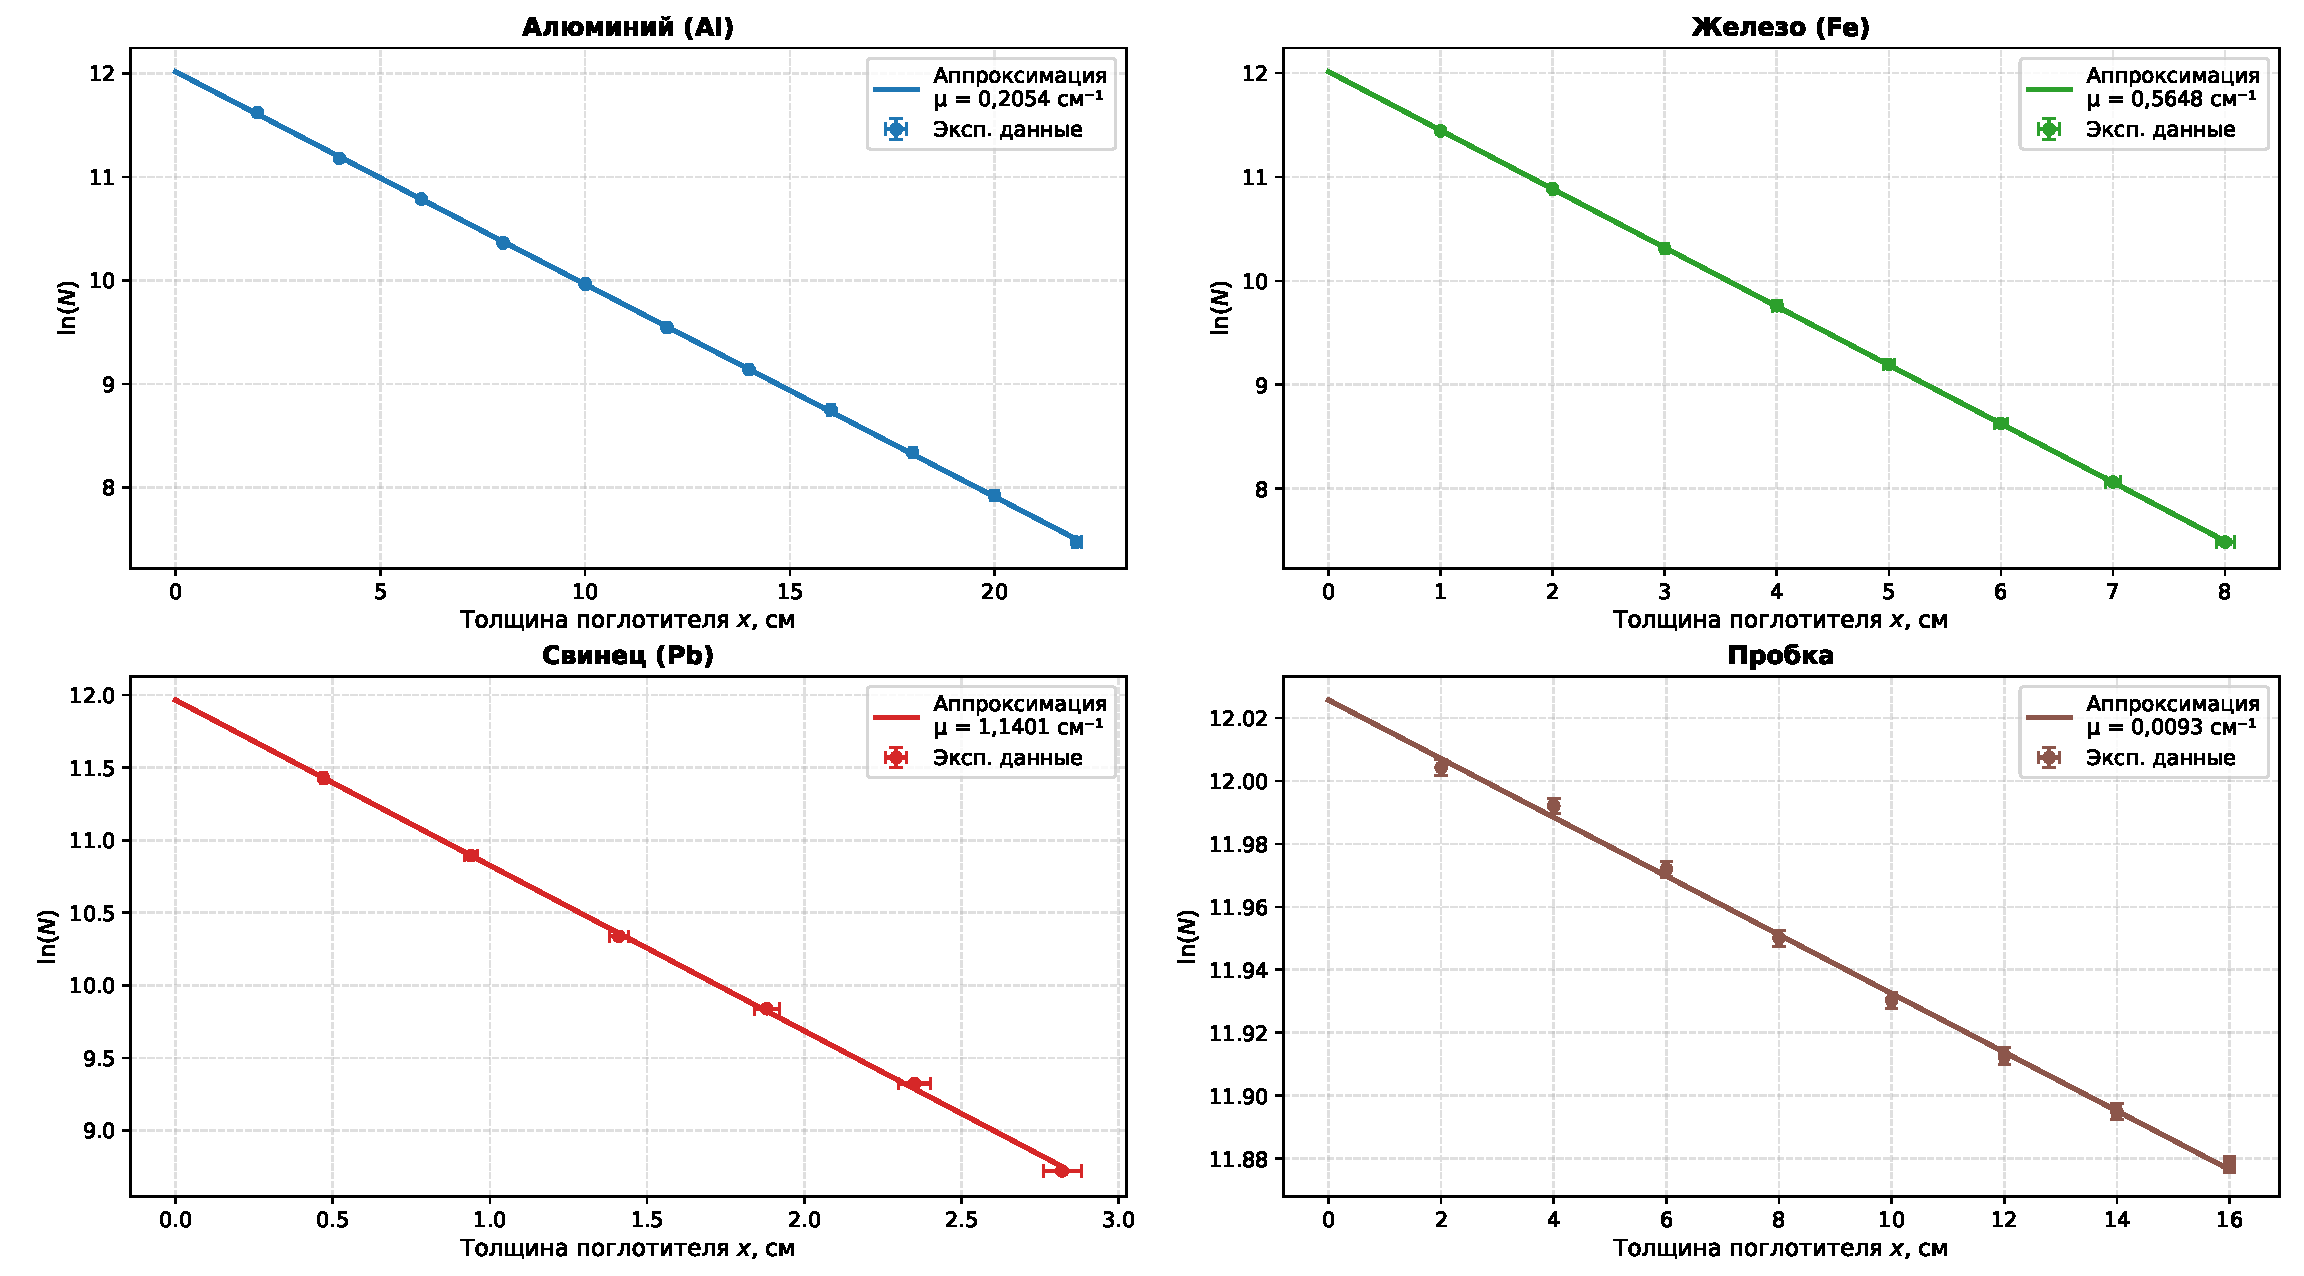
\includegraphics[width=\textwidth]{1.pdf}
    \caption{Зависимость натурального логарифма интенсивности $\ln(N)$ от толщины поглотителя $x$ для каждого материала в отдельности.}
    \label{fig:attenuation_individual}
\end{figure}

\begin{figure}[h!]
    \centering
    % Убедитесь, что имя файла совпадает с тем, что сохраняет ваш Python-скрипт
    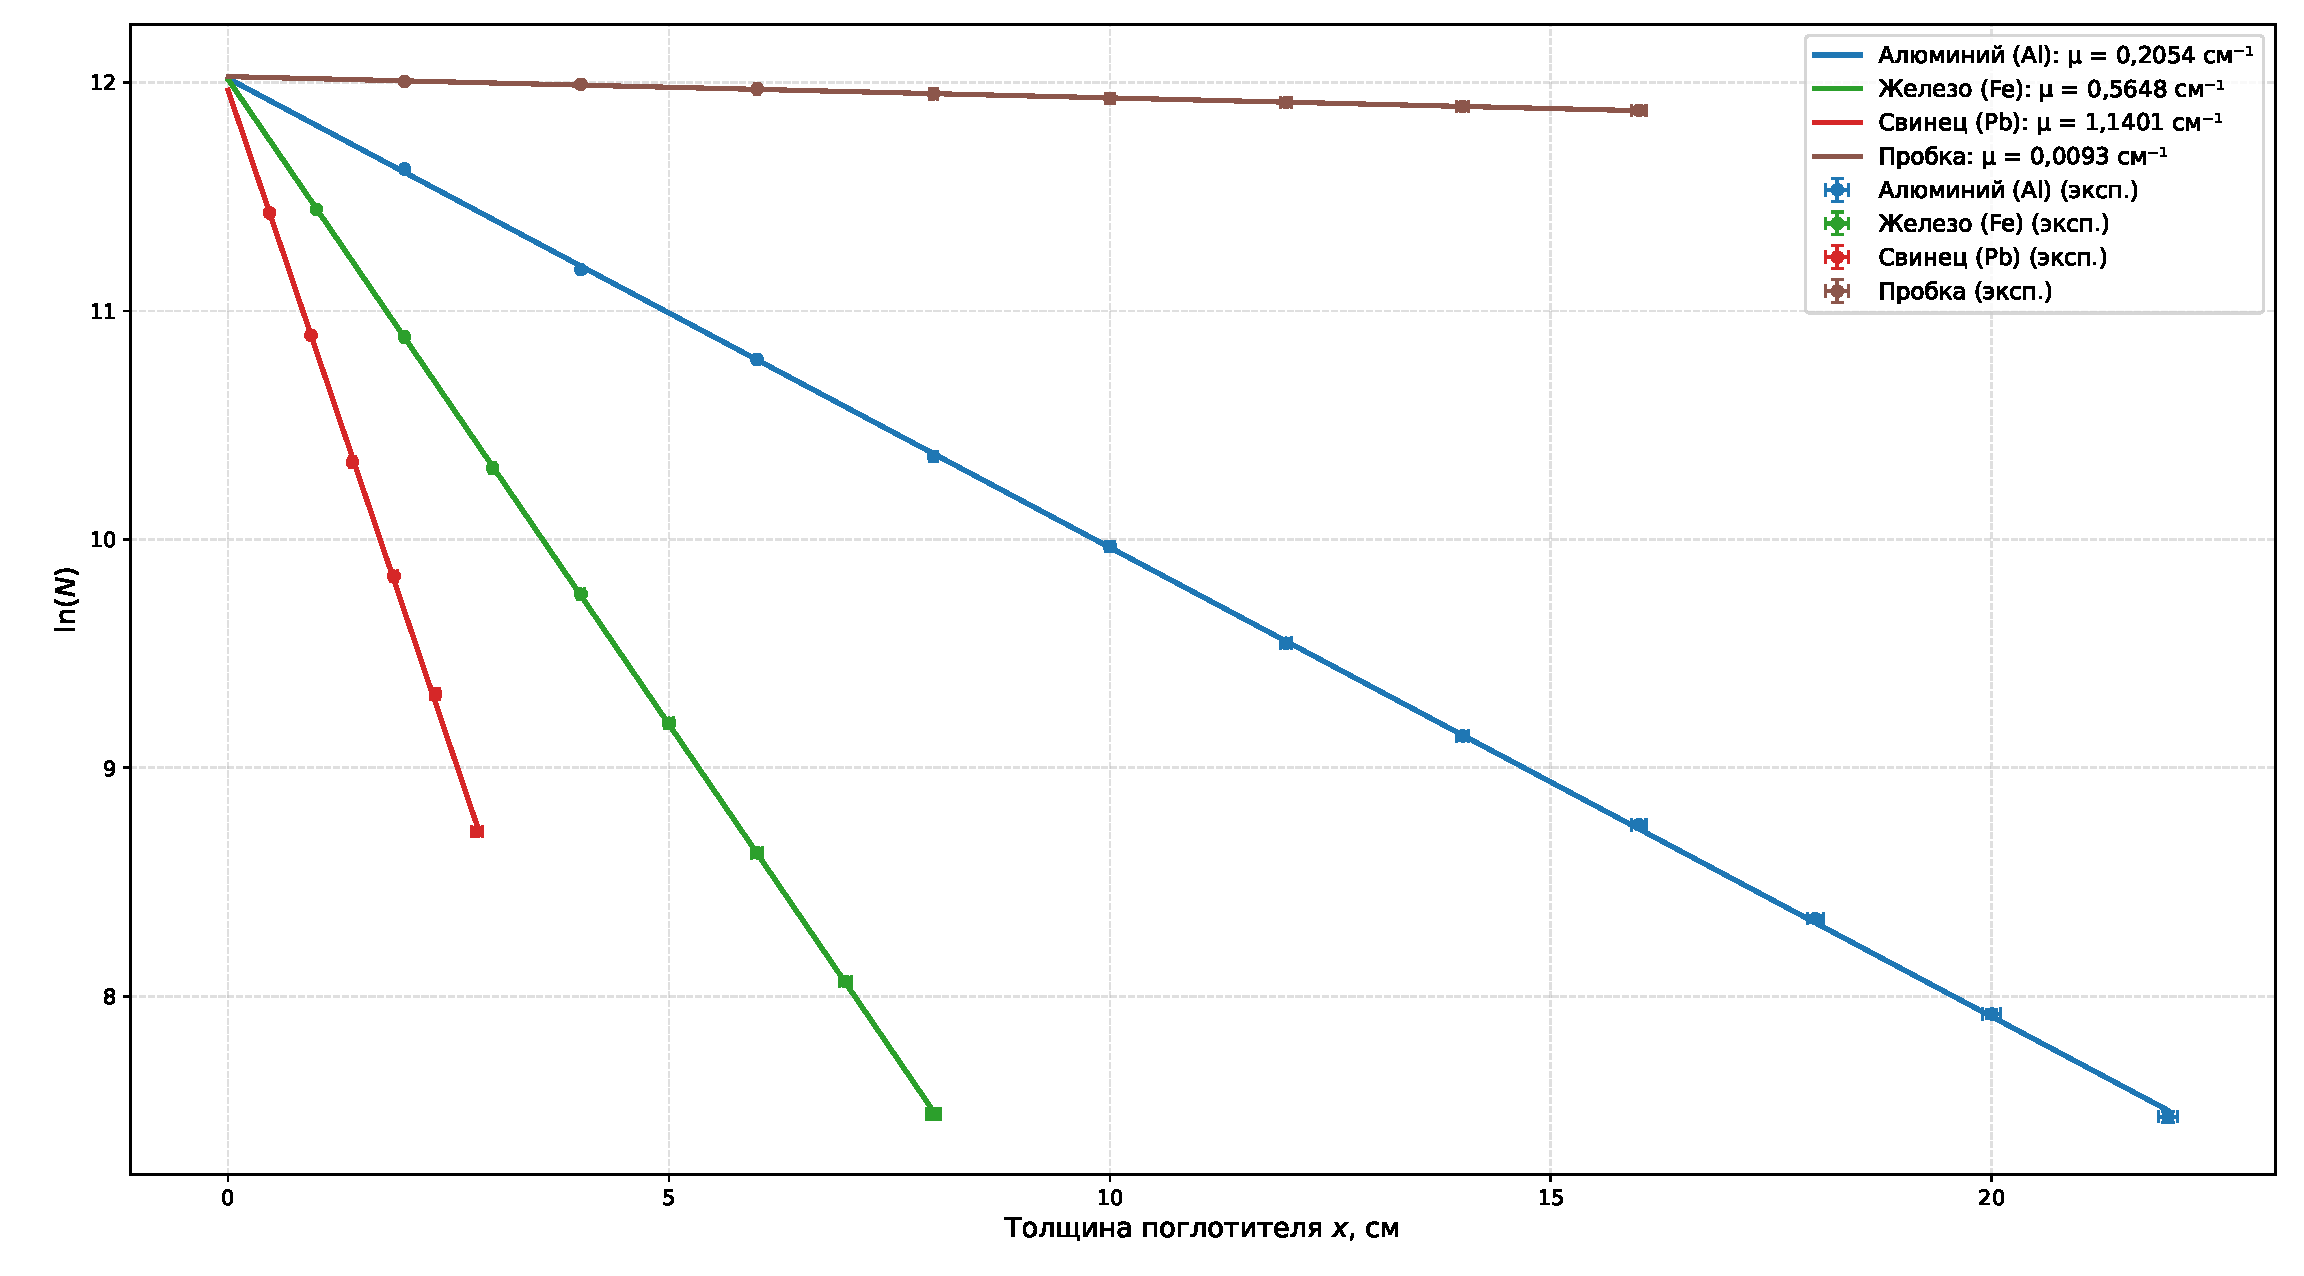
\includegraphics[width=0.9\textwidth]{2.pdf}
    \caption{Сравнительный график зависимости $\ln(N)$ от толщины поглотителя $x$ для всех исследованных материалов на одной координатной плоскости.}
    \label{fig:attenuation_combined}
\end{figure}
% Погрешность определения $\mu$ ($\Delta \mu$) рассчитывалась как стандартная ошибка наклона прямой при линейной регрессии:
% \begin{equation}
%     \Delta \mu = \sqrt{ \frac{1}{n-2} \cdot \frac{\sum\limits_{i=1}^{n} (\ln N_i - \widehat{\ln N_i})^2}{\sum\limits_{i=1}^{n} (x_i - \bar{x})^2} },
% \end{equation}
% где $n$ --- количество измерений, $\widehat{\ln N_i}$ --- значение, предсказанное аппроксимирующей прямой, $\bar{x}$ --- среднее значение толщины.

Массовый коэффициент ослабления $\mu'$ вычислялся по формуле $\mu' = \mu / \rho$, где $\rho$ --- табличная плотность вещества. %Погрешность $\Delta \mu'$ находилась по формуле переноса погрешностей (с учётом относительной погрешности табличной плотности $\Delta \rho / \rho \approx 1\,\%$):
% \begin{equation}
%     \Delta \mu' = \mu' \sqrt{ \left( \frac{\Delta \mu}{\mu} \right)^2 + \left( \frac{\Delta \rho}{\rho} \right)^2 }.
% \end{equation}

Результаты расчётов представлены в таблице~\ref{tab:mu_results}:

\begin{table}[h!]
\centering
\caption{Линейные и массовые коэффициенты ослабления $\gamma$-излучения}
\label{tab:mu_results}
\renewcommand{\arraystretch}{1.3}
\begin{tabular}{|l|c|c|}
\hline
\textbf{Материал} & \textbf{$\mu \pm \Delta \mu$, см$^{-1}$} & \textbf{$\mu' \pm \Delta \mu'$, см$^2$/г} \\
\hline
Алюминий (Al) & $0{,}2054 \pm 0{,}0015$ & $0{,}0761 \pm 0{,}0007$ \\
\hline
Железо (Fe)   & $0{,}5648 \pm 0{,}0050$ & $0{,}0718 \pm 0{,}0008$ \\
\hline
Свинец (Pb)   & $1{,}1401 \pm 0{,}0120$ & $0{,}1005 \pm 0{,}0012$ \\
\hline
Пробка        & $0{,}0093 \pm 0{,}0008$ & $0{,}0389 \pm 0{,}0040$ \\
\hline
\end{tabular}
\end{table}












\subsection*{Определение энергии $\gamma$-квантов источника}

% Используя найденные значения массовых коэффициентов ослабления для свинца, железа и алюминия и сопоставляя их с табличными зависимостями $\mu'(E)$ (таблица V.4 из Приложения V методического пособия), определим энергию $\gamma$-квантов, испускаемых источником.

% Экспериментальные значения $\mu'$:
% \begin{itemize}
%     \item для алюминия: $\mu'_{\text{Al}} = 0{,}0761 \pm 0{,}0007$~см$^2$/г;
%     \item для железа: $\mu'_{\text{Fe}} = 0{,}0718 \pm 0{,}0008$~см$^2$/г;
%     \item для свинца: $\mu'_{\text{Pb}} = 0{,}1005 \pm 0{,}0012$~см$^2$/г.
% \end{itemize}

Согласно табличным данным, указанным значениям массовых коэффициентов ослабления соответствуют энергии $\gamma$-квантов порядка $0{,}6$~МэВ для всех трёх материалов. Полученный результат согласуется с ожидаемым значением энергии $E_\gamma = 0{,}662$~МэВ, характерным для радиоактивного изотопа $^{137}$Cs. Небольшое расхождение объясняется конечной геометрией пучка и статистическими погрешностями измерений.



\section*{Вывод}

В ходе выполнения лабораторной работы был экспериментально исследован процесс ослабления $\gamma$-излучения в различных веществах (алюминии, железе, свинце и пробке). Методом линейной аппроксимации зависимости натурального логарифма интенсивности от толщины поглотителя были определены линейные ($\mu$) и массовые ($\mu'$) коэффициенты ослабления.

Сопоставление полученных экспериментальных значений массовых коэффициентов ослабления с табличными зависимостями $\mu'(E)$ позволило определить среднюю энергию $\gamma$-квантов исследуемого источника: $E_\gamma \approx 0{,}6$~МэВ. Это значение с учётом экспериментальных и систематических погрешностей соответствует энергии радиоактивного изотопа $^{137}$Cs ($E_{\text{табл}} = 0{,}662$~МэВ), что подтверждает правильность проведённых измерений.

Отдельно следует отметить, что экспериментальное значение коэффициента ослабления для свинца отклоняется от табличного в большей степени, чем для алюминия и железа. Это систематическое расхождение обусловлено следующими причинами: %рядом физических факторов, специфичных для материалов с высокой плотностью и большим атомным номером ($Z=82$):

\begin{enumerate}
    \item \textbf{Нарушение условий «хорошей геометрии» (эффект накопления).} Теоретический закон $I = I_0 e^{-\mu x}$ строго выполняется для идеально узкого пучка, когда любой акт взаимодействия выводит фотон из пучка. В реальной установке детектор имеет конечные размеры. В свинце, обладающем высоким сечением взаимодействия, велика вероятность того, что фотон испытает комптоновское рассеяние на малый угол или многократное рассеяние и всё же попадёт в детектор. Это приводит к искусственному завышению измеренной интенсивности и, как следствие, к занижению расчётного значения $\mu$.
    
    \item \textbf{Регистрация вторичного характеристического излучения.} При взаимодействии $\gamma$-квантов со свинцом за счёт фотоэффекта происходит ионизация внутренних оболочек атомов. При заполнении образовавшихся вакансий испускаются кванты характеристического рентгеновского излучения свинца (с энергиями $\sim 75$--$85$~кэВ). Эти вторичные кванты легко проходят через оставшуюся часть поглотителя, достигают детектора и регистрируются как прошедшие сквозь него, что также занижает истинный коэффициент ослабления.
    
    % \item \textbf{Геометрический фактор.} Поскольку свинец сильно поглощает излучение, используются тонкие пластины (порядка нескольких миллиметров). Абсолютная погрешность измерения их толщины ($\Delta x = 0{,}01$~см) даёт большую относительную погрешность по сравнению с толстыми пластинами алюминия или пробки.
\end{enumerate}

Таким образом, поставленные в работе задачи выполнены, а полученные результаты подтверждают экспоненциальный характер ослабления $\gamma$-излучения и зависимость коэффициента ослабления от атомного номера и плотности вещества.







\section*{Ответ на вопрос о сцинтилляции чистого NaI}

Утверждение о том, что чистый (нелегированный) NaI плохо сцинтиллирует, справедливо в первую очередь для его использования при комнатной температуре в макроскопических объёмах. Однако чистый NaI обладает собственной люминесценцией, и при определённых условиях он работает весьма эффективно.

\subsubsection*{Механизм сцинтилляции чистого NaI}

В чистом кристалле NaI сцинтилляция происходит за счёт \textbf{собственной люминесценции}, связанной с образованием и рекомбинацией \textit{самолокализованных экситонов} (Self-Trapped Exciton, STE). Процесс развивается следующим образом:

\begin{enumerate}
    \item Гамма-квант выбивает электрон из валентной зоны в зону проводимости, оставляя после себя дырку.
    \item В щелочно-галоидных кристаллах дырка не остаётся свободной, а захватывает соседний ион галогена ($\text{I}^-$), образуя молекулярный ион $\text{I}_2^-$, так называемый $V_k$-центр.
    \item Электрон из зоны проводимости притягивается к этому положительному $V_k$-центру, образуя связанное состояние --- самолокализованный экситон (STE).
    \item При рекомбинации экситона (переходе в основное состояние) испускается фотон.
\end{enumerate}

Энергия этого перехода соответствует ультрафиолетовому диапазону: максимум спектра испускания чистого NaI лежит в области $\lambda \approx 290\text{--}300$~нм. Именно здесь кроется главная проблема: спектр испускания чистого NaI сильно перекрывается с краем его собственного поглощения. Возникающий УФ-фотон с высокой вероятностью поглощается соседним атомом кристалла ещё до того, как покинет его (эффект \textbf{самопоглощения}). Это и есть причина, по которой в методичке указано, что возникающее излучение должно сильно поглощаться в сцинтилляторе.

\subsubsection*{Условия, при которых чистый NaI сцинтиллирует эффективно}

Чтобы обойти проблему самопоглощения и низкого светового выхода, чистый NaI используют при соблюдении следующих условий:

\begin{enumerate}
    \item \textbf{Низкие (криогенные) температуры.} При охлаждении кристалла (например, до температуры жидкого азота, $77$~К, и ниже) резко подавляется безызлучательная рекомбинация (термическое тушение люминесценции). Световой выход чистого NaI при $77$~К возрастает в разы и может достигать $40\text{--}50\,\%$ от светового выхода NaI(Tl) при комнатной температуре, а в некоторых конфигурациях даже сравниваться с ним. Именно поэтому чистый NaI исторически применялся в специализированных физических экспериментах (например, в детекторах тёмной материи и нейтрино), где важна радиационная чистота кристалла.
    
    \item \textbf{Малые геометрические размеры кристалла.} Если кристалл сделать очень тонким или маленьким, вероятность того, что УФ-фотон будет поглощён внутри кристалла до выхода наружу, значительно снижается. Это позволяет собрать достаточное количество света даже при наличии самопоглощения.
    
    \item \textbf{Задачи, требующие сверхбыстрого времени отклика.} У чистого NaI время высвечивания составляет всего $\sim 10\text{--}20$~нс, тогда как у активированного таллием NaI(Tl) оно равно $\sim 230$~нс. Если стоит задача регистрации быстрых совпадений частиц (например, в физике высоких энергий), и при этом используются специальные ФЭУ с кварцевым окном (пропускающим УФ) и фотокатодом, чувствительным к ультрафиолетовому диапазону, чистый NaI может быть предпочтительнее именно из-за своего быстродействия, несмотря на меньший общий световой выход.
\end{enumerate}

% \subsubsection*{Краткий вывод}

% Чистый NaI обладает собственной сцинтилляцией за счёт рекомбинации самолокализованных экситонов (STE) с испусканием УФ-фотонов ($\lambda \approx 300$~нм). Основная проблема при комнатной температуре --- сильное самопоглощение этого излучения внутри самого кристалла. Однако чистый NaI эффективно сцинтиллирует при низких (криогенных) температурах, где термическое тушение подавлено, а также в малоразмерных кристаллах, где путь пробега фотона мал. Кроме того, чистый NaI имеет очень малое время высвечивания ($\sim 10$~нс против $\sim 230$~нс у NaI(Tl)), что делает его полезным для задач на быструю временную селекцию при использовании ФЭУ, чувствительных к ультрафиолету.






\section*{Детектор на ядерных фотоэмульсиях}

\subsubsection*{Принцип работы}

Ядерная фотоэмульсия --- это специализированный тип фотографической эмульсии, предназначенный для регистрации треков заряженных частиц. В отличие от обычной фотоплёнки, в которой размер кристаллов галогенида серебра ($\text{AgBr}$) составляет несколько микрометров, в ядерных эмульсиях используются ультрадисперсные кристаллы размером $0{,}1\text{--}0{,}3$~мкм. Это позволяет достичь пространственного разрешения порядка $1$~мкм, что делает эмульсию фактически трёхмерным трековым детектором с нанометровой точностью.

Физический механизм регистрации следующий. Пролетающая через эмульсию заряженная частица ионизирует атомы брома в кристаллах $\text{AgBr}$, выбивая из них электроны. Эти электроны захватываются ионами серебра $\text{Ag}^+$, превращая их в нейтральные атомы $\text{Ag}^0$. Таким образом вдоль траектории частицы образуется скрытое изображение --- цепочка кристаллов, содержащих центры чувствительности. При последующей химической проявке (по аналогии с обычной фотографией) эти кристаллы восстанавливаются до металлического серебра, образуя видимую под микроскопом цепочку тёмных зёрен. Плотность зёрен на единицу длины трека (так называемая \textit{зернистость трека}) пропорциональна квадрату заряда частицы и обратно пропорциональна квадрату её скорости ($\propto Z^2/\beta^2$), что позволяет идентифицировать тип частицы.

\subsubsection*{Что регистрирует и измеряет}

Ядерная фотоэмульсия регистрирует траектории заряженных частиц (протонов, мезонов, ядер, электронов) с высокой точностью. Измеряемыми величинами являются:
\begin{itemize}
    \item \textbf{Длина пробега} частицы до остановки --- позволяет определить её начальную кинетическую энергию;
    \item \textbf{Плотность зёрен} вдоль трека --- даёт информацию о заряде и скорости частицы;
    \item \textbf{Углы рассеяния} и вершины распадов --- позволяют изучать процессы взаимодействия частиц и идентифицировать короткоживущие частицы по характерным вилкам распада;
    \item \textbf{Множественное кулоновское рассеяние} --- по углу отклонения трека на малых участках можно оценить импульс частицы.
\end{itemize}

\subsubsection*{Области применения}

Исторически ядерные эмульсии сыграли ключевую роль в физике элементарных частиц. Именно с их помощью были открыты $\pi$-мезон и гиперон $\Omega^-$.% За эти открытия были присуждены Нобелевские премии.

В современной физике ядерные эмульсии используются в экспериментах, требующих сверхвысокого пространственного разрешения:
\begin{itemize}
    \item \textbf{Эксперимент OPERA} (Гран-Сассо, Италия) --- первое прямое наблюдение осцилляций нейтрино через регистрацию рождения $\tau$-лептона при взаимодействии $\nu_\tau$ с ядром. Именно эмульсионные детекторы позволили зафиксировать микроскопическую вилку распада $\tau$-лептона с длиной пробега менее миллиметра.
    \item \textbf{Эксперимент NEWSdm} --- поиск частиц тёмной материи (вимпов) по характерным коротким трекам ядер отдачи.
    \item \textbf{Космическая дозиметрия} --- эмульсионные детекторы используются на МКС и в межпланетных миссиях для регистрации тяжёлых ядер космических лучей.
    \item \textbf{Медицинская физика} --- в протонной и ионной терапии для прецизионного контроля распределения дозы в фантомах.
\end{itemize}

\subsubsection*{Преимущества}

\begin{enumerate}
    \item \textbf{Сверхвысокое пространственное разрешение} ($\sim 1$~мкм) --- недостижимое для большинства электронных детекторов.
    \item \textbf{Пассивность и автономность} --- не требует электропитания, охлаждения или считывания в реальном времени; может работать годами.
    \item \textbf{Трёхмерность трека} --- вся информация о траектории частицы сохраняется в объёме эмульсии и может быть восстановлена послойно.
    \item \textbf{Интегрирующий характер} --- регистрирует все частицы, прошедшие через детектор за всё время экспозиции, без мёртвого времени.
    \item \textbf{Радиационная стойкость} --- в отличие от полупроводниковых детекторов, не деградирует под действием высоких доз облучения.
\end{enumerate}

\subsubsection*{Недостатки}

\begin{enumerate}
    \item \textbf{Трудоёмкость анализа} --- считывание треков требует автоматизированных микроскопов с высоким разрешением и сложного программного обеспечения для распознавания образов.
    \item \textbf{Отсутствие сигнала в реальном времени} --- невозможно использовать для триггерных систем или онлайн-мониторинга; результат доступен только после проявки.
    \item \textbf{Чувствительность к условиям хранения} --- эмульсии требуют контроля температуры и влажности, иначе происходит термическое засвечивание (рост фона).
    \item \textbf{Ограниченный динамический диапазон} --- при очень высоких плотностях треков зёрна сливаются, и треки становятся неразличимыми.
    \item \textbf{Невозможность регистрации нейтральных частиц} --- как и любой трековый детектор, эмульсия чувствительна только к заряженным частицам; нейтральные частицы регистрируются лишь косвенно, по вторичным трекам продуктов их взаимодействия.
\end{enumerate}

Таким образом, детектор на ядерных фотоэмульсиях, несмотря на свою более чем вековую историю, остаётся уникальным инструментом в тех задачах, где критически важно микронное пространственное разрешение и трёхмерная реконструкция треков.

\begin{figure}[h!]
    \centering
    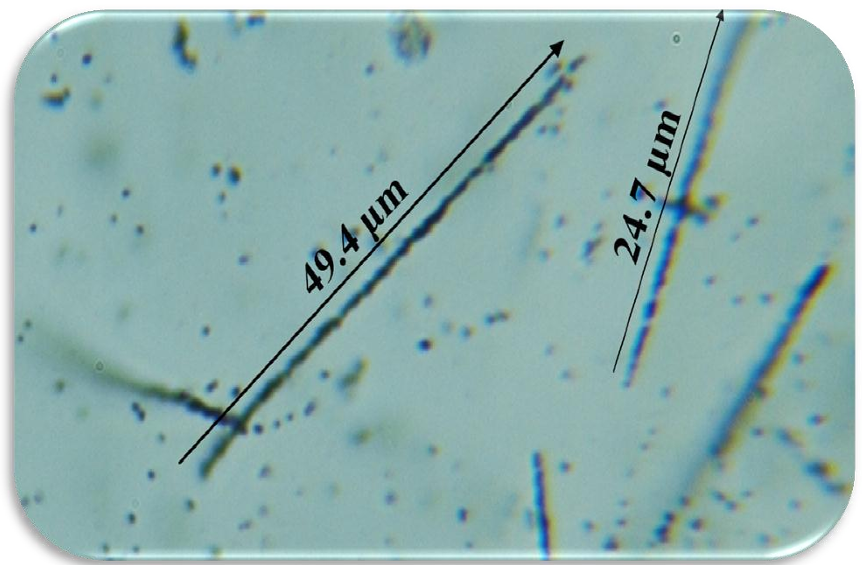
\includegraphics[width=0.8\textwidth]{4.png}
    \caption{Треки $\alpha$-частиц в ядерной фотоэмульсии. Стрелками указаны длины пробегов частиц (49{,}4~мкм и 24{,}7~мкм). Различная плотность зёрен вдоль трека отражает изменение скорости частицы: по мере торможения плотность ионизации растёт, что приводит к увеличению числа проявленных зёрен серебра на единицу длины.}
    \label{fig:alpha_track}
\end{figure}

\vspace{0.5cm}

\begin{figure}[h!]
    \centering
    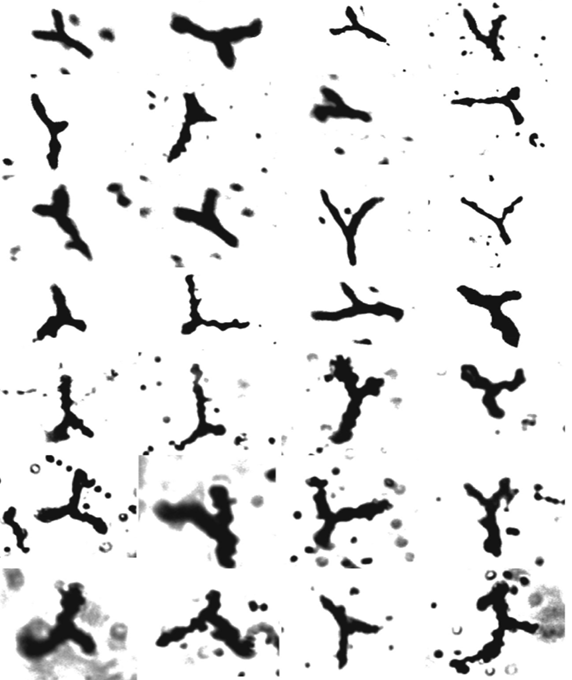
\includegraphics[width=0.9\textwidth]{5.png}
    \caption{Примеры событий тройного деления ядер, зарегистрированных в ядерной фотоэмульсии. Характерные ``вилки'' распада позволяют идентифицировать короткоживущие частицы и изучать процессы взаимодействия. Именно анализ подобных изображений привёл к открытию $\pi$-мезона и гиперона $\Omega^-$.}
    \label{fig:ternary_fission}
\end{figure}

\vspace{0.5cm}

\begin{figure}[h!]
    \centering
    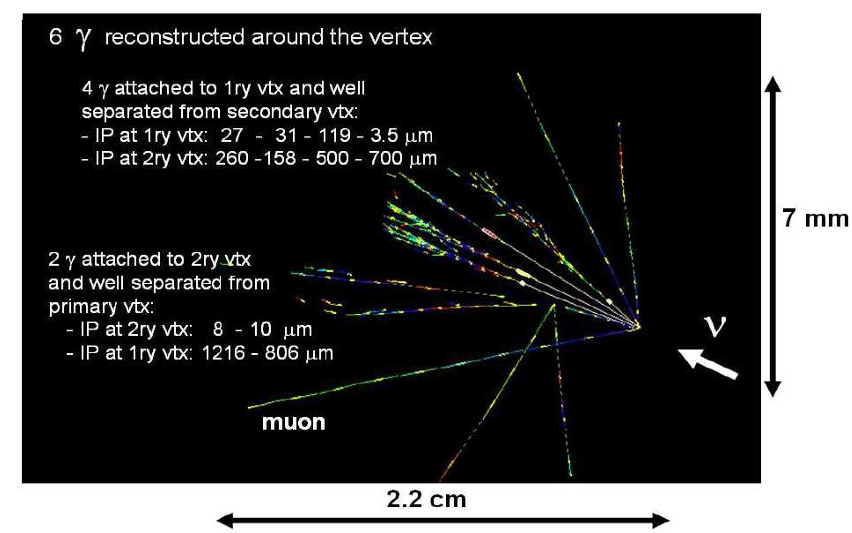
\includegraphics[width=0.85\textwidth]{6.png}
    \caption{Реконструкция взаимодействия мюонного нейтрино ($\nu_\mu$) в эмульсионном детекторе (эксперимент OPERA). Белая стрелка указывает направление пучка нейтрино. Мюон и несколько гамма-квантов хорошо разделяются по параметрам прицельного расстояния относительно первичной и вторичной вершин. Подобная трёхмерная реконструкция треков с микронным разрешением позволила впервые напрямую зарегистрировать рождение $\tau$-лептона и доказать осцилляции нейтрино.}
    \label{fig:neutrino_interaction}
\end{figure}


\end{document}